\documentclass{subfiles}

\begin{document}
    \subsubsection*{Das Doppelspaltexperiment}
        \marginnote{\textbf{\textit{VL 9}}\\17.05.2023,\\08:15}
        Als Paradebeispiel dieses Dualismus gilt das berühmte \href{https://de.wikipedia.org/wiki/Doppelspaltexperiment}{\emph{Doppelspaltexperiment}}. Welche Objekte hierbei verwendet werden, stellt sich als vielfältig heraus: von makroskopischen Teilchen, klassische Wellen oder auch Quantenobjekte selbst. 
        \begin{figure}[H]
            \centering
            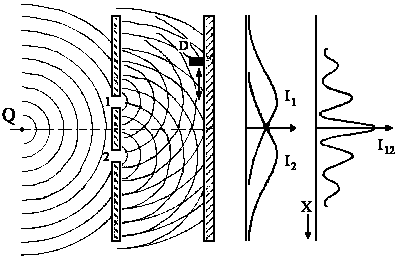
\includegraphics[width=5cm]{Bilddateien/Doppelspalt.png}
            \caption{Der Aufbau und Ablauf des Doppelspaltexperimentes im Wellenbild aus \cite{tubs:Doppelspalt}.}
        \end{figure}
        Die Amplitude im Teilchenfall ergibt sich dabei durch $I_1 = \abs{A_1}^2$, im Wellenfall dagegen aus $I = \abs{A_1+A_2}^2$. 
        \begin{Aufgabe}
            \nr{} Berechne die Wellenintensität für zwei komplexe Amplituden $\psi_1,\psi_2\in\C$. 
        \end{Aufgabe}
        \begin{Experiment}{Ein Doppelspaltexperiment}
            \label{Ub:Doppelspaltexperiment}
            Wir wollen nun die Maxima der Schirmverteilung untersuchen: Hierzu ziehen wir einen Sensor zur Photonenmessung pro Zeitintervall mit verschiebbarer Position $x$ über den Schirm. Die Messwerte suggerieren den erwarteten Verlauf der Wellenintensität.
        \end{Experiment}

    
\end{document}